\documentclass[11pt,a4paper]{article}

\usepackage[utf8]{inputenc}
\usepackage[english]{babel}
\usepackage[T1]{fontenc}

\usepackage{amsmath,amssymb,amsfonts}
\usepackage{hyperref}
\usepackage{graphicx}

\title{Computational Geometry - Range Searching}
\author{Philip Munksgaard \\ Sebastian Paaske Tørholm \\ Ejnar Håkonsen}

\begin{document}
\maketitle

\section{Exercise 5.1}

We use the first rule of the master theorem~\cite{Cormen theorem 4.1}
to solve the recurrence. Since $a=2, b=4, f(n)=2$, we get that $\log_b a
= \frac{1}{2}$ and thus we get $Q(n) = \Theta(\sqrt{n})$.

Given that $Q(n) = \Theta(\sqrt{n})$, we also have $Q(n) = \Omega(\sqrt{n})$
as desired.

\begin{figure}[h!]
    \centering
    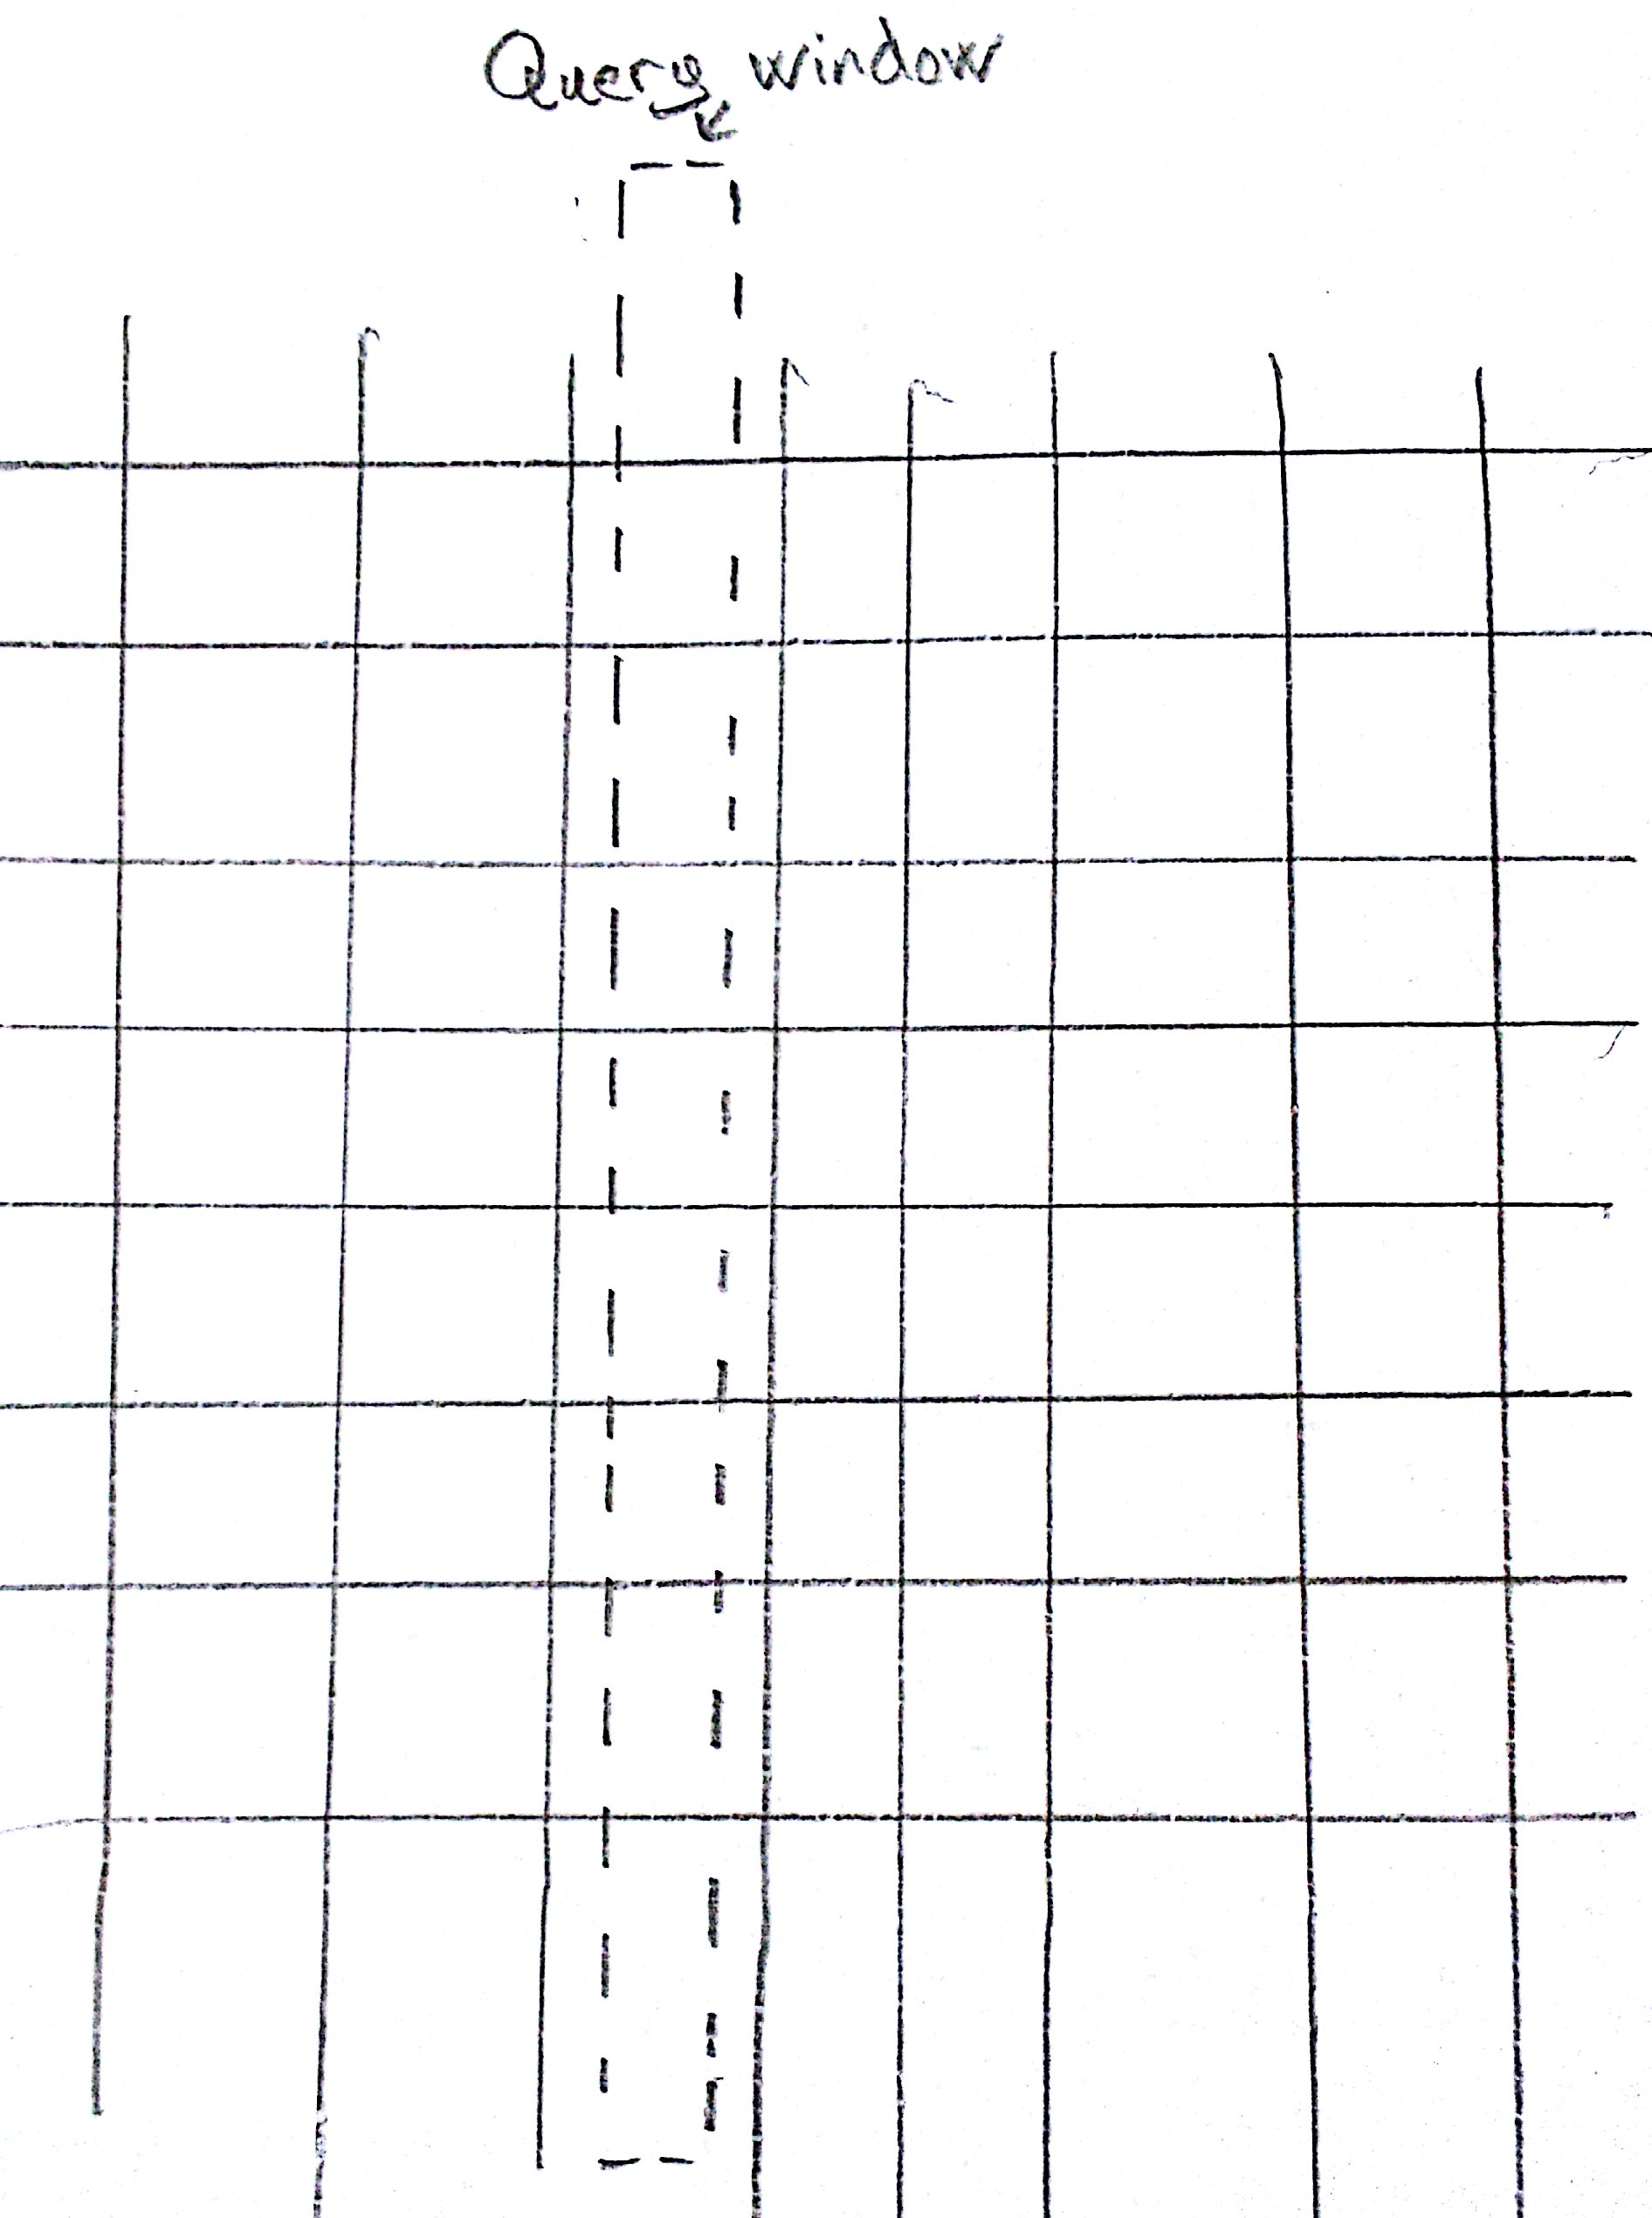
\includegraphics[width=.6\textwidth]{tegning-ex51.jpg}
    \caption{Construction for the worst case in exercise 5.1}
    \label{tegning-ex51}
\end{figure}

We can see an example of such a worst case by constructing a $m \times m$ grid
of evenly spaced points. It's easy to convince oneself that the splitting of
the plane done by the $kd$-tree will contain the lines of the grid.
\footnote{Minor tweaking of $x$ and $y$ coordinates is necessary to make
them distinct, but the idea should hold nonetheless.}

Let us then consider a query window starting above the grid, and ending below it,
placed such that it doesn't contain any points. (See \autoref{tegning-ex51})
This window will intersect at least $m$ lines, and overlap with at least $m+1$
regions. If we let $n = m^2$, we get $\sqrt{n}+1$ regions we must check, and
as such is an example of the worst case.

\section{Exercise 5.10}

\end{document}

